\section{Secure Functionalities}
\label{sec:technique-in-depth}

\subsection{Secure device Discovery}
 Device discovery serves two functions: 1) it is used in the context of discovering neighboring Embedded systems to form routing paths, where existing mechanims can be use; 2) for device onboarding, on which we focus here. During onboarding, the Embedded system passes its device-level information (such as manufacturer-ID and model number) and application-level information (such as service type and data type) to the upstream devices. But, if the device is required to have a globally unique ICN ID, it can be provided one by the naming service.\par
 n the name-based ICN approaches where device identity is not needed, a device can publish within the name scope of the aggregator.In most IoT systems, devices interact with the aggregator for data or information processing or aggregation, hence there is no direct communication between devices under an aggregator. If in some set-up devices under the aggregator need to communicate with each other a scalable mechanism is to allow direct neighbors to communicate with each other while others communicate through the aggregator.
 
 Fig. \ref{fig:Secure device Discovery}.
 \begin{figure}[h]
	\centering
	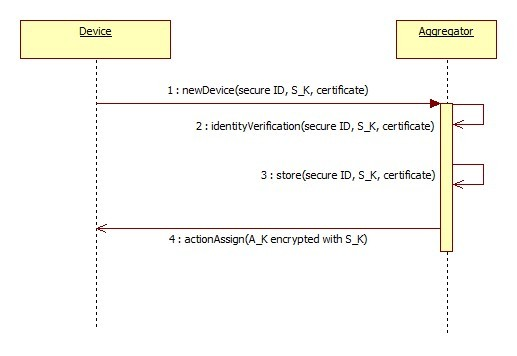
\includegraphics[width=0.8\linewidth]{Figures/Secure-device-discovery-with-pre-load-secure-keys.png}
	\caption[]{Secure device Discovery}
	\label{fig:Secure device Discovery}
\end{figure}

\subsection{Secure service Discovery}
Secure service Discovery Fig. \ref{fig:Secure service Discovery}.
 \begin{figure}[h]
	\centering
	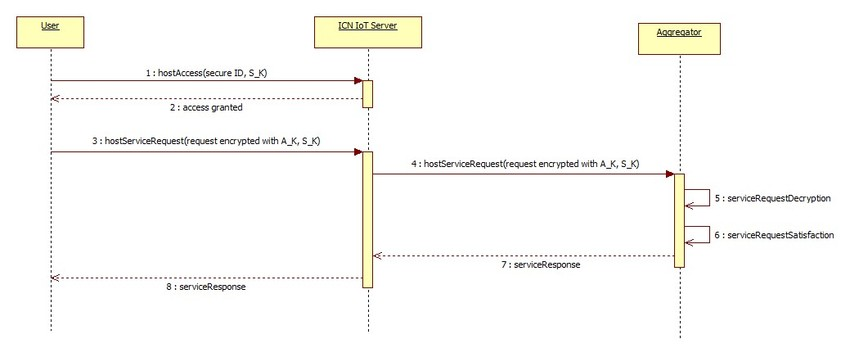
\includegraphics[width=0.8\linewidth]{Figures/Secure-service-discovery.png}
	\caption[]{Secure service Discovery}
	\label{fig:Secure service Discovery}
\end{figure}
\par
\subsection{Secure naming service}
If a device needs a global unique name/ID, but does not have one, it may request the naming service to obtain one after it is authenticated. Alternatively, the IoT domain (LSG or aggregator) may determine ID (name) for an authenticated device is required based on the policy. The proposed naming process works as follows. After a device has been authenticated, it may request an ID from the naming service (or the aggregator, if it can give the device a locally unique name). It sends a ID request (IDReq) to the naming service or aggregator. If the aggregator can accept request to give a unique name to the device, it will do that.\par
 Fig. \ref{fig:Secure naming service}.
 \begin{figure}[h]
	\centering
	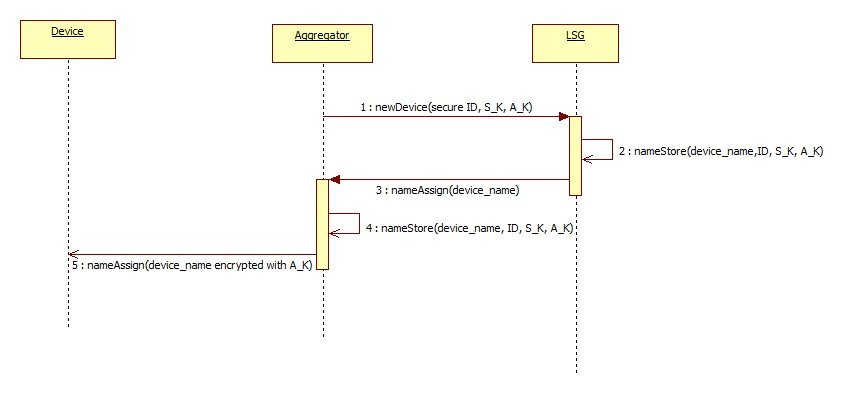
\includegraphics[width=0.8\linewidth]{Figures/Secure-naming-service.jpg}
	\caption[]{Secure naming service}
	\label{fig:Secure naming service}
\end{figure}
\par
\subsection{User registration}
User Registration.
 A user, who wants to access/subscribe to a service, has to perform the registration operation by sending information that depends on the specific application domain to the IoT server. The information can be secured with the help of the PKI infrastructure. Upon successful registration the IoT server securely transmits an identifier, a user signature key SK (to be used to sign messages), a user encryption key EK (to communicate data confidentially), and an access password to the user in an encrypted message. Upon reception of the message, the user accesses the system to modify his/her password (function changePassword). With respect to existing secure application-layer solutions, a further benefit of the presented approach is the introduction of a second level of security, represented by the use of a temporary password (immediately replaced) and a couple of keys (signature SK and encryption EK), which is well suited for the heterogeneous and distributed IoT environment.
Fig. \ref{fig:User registration}.
 \begin{figure}[h]
	\centering
	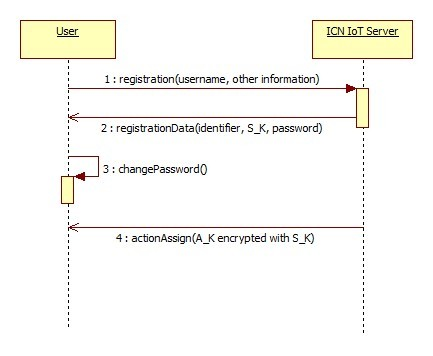
\includegraphics[width=0.8\linewidth]{Figures/User-registration-secure-subscribe.png}
	\caption[]{User registration}
	\label{fig:User registration}
\end{figure}
\par
\subsection{Secure content discovery}
Secure content discovery Fig. \ref{fig:Secure content discovery}.
 \begin{figure}[h]
	\centering
	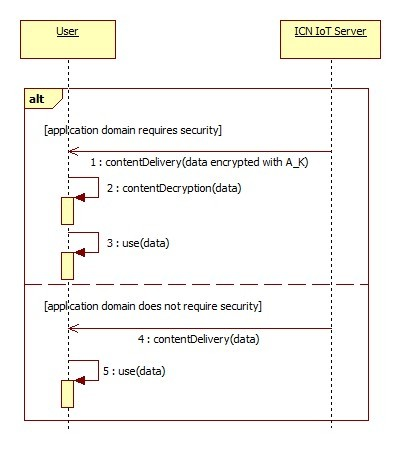
\includegraphics[width=0.8\linewidth]{Figures/Secure-content-delivery-user.png}
	\caption[]{Secure content discovery}
	\label{fig:Secure content discovery}
\end{figure}
\par
